\section{Teorema de Stokes}

El teorema de Stokes relaciona la circulación de un campo vectorial sobre una curva cerrada en el espacio con el flujo de su rotacional a través de una superficie cuya frontera es esa curva. Generaliza la forma de circulación del teorema de Green y permite elegir entre una integral de línea y una integral de superficie según la geometría y el campo.

\subsection{Rotacional y orientación de la frontera}

\begin{mydefinition}{Rotacional de un campo vectorial}
Si $\mathbf F=\langle P,Q,R\rangle$ es de clase $C^1$ en un abierto $U\subseteq\mathbb R^3$, su rotacional es
\[
\nabla\times\mathbf F
=\left\langle R_y-Q_z,\ P_z-R_x,\ Q_x-P_y\right\rangle.
\]
\end{mydefinition}
La circulación $\oint_C\mathbf F\cdot d\vec r$ mide la acumulación de la componente tangencial del campo a lo largo del recorrido cerrado. El rotacional describe su circulación local por unidad de área orientada; la relación precisa se obtiene del teorema de Stokes.

\begin{mydefinition}{Orientación inducida en la frontera}
Sea $S$ una superficie orientada mediante una normal unitaria $\mathbf n$. La orientación positiva de $C=\partial S$ es la compatible con la regla de la mano derecha: los dedos siguen el sentido de recorrido de la frontera y el pulgar señala el lado de la normal. Localmente, al avanzar por la frontera con la cabeza en el sentido de $\mathbf n$, la superficie queda a la izquierda.
\end{mydefinition}

\begin{center}
\begin{minipage}{.9\textwidth}
\centering
\begingroup\shorthandoff{>}
\def\manoNormal{\mathbf n}\def\manoRecorrido{C\text{ positivo}}
% Mano derecha con dedos curvados; etiquetas definidas localmente.
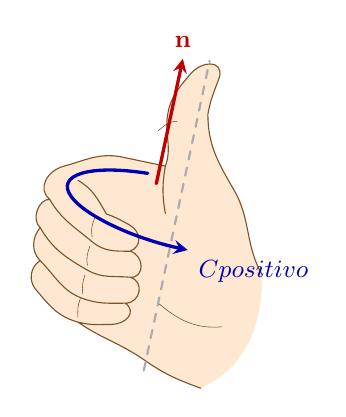
\begin{tikzpicture}[scale=.6,every node/.style={font=\small},>=stealth,
 line join=round,line cap=round]
\fill[orange!18] (2.9,-1.1)--(.85,1.2)--(-1.3,1.2)--(-1,-2.1)
--(.4,-2.9)--(1.6,-3.5) to[out=25,in=-90] cycle;
\draw[fill=orange!18,draw=brown!65!black] (2.9,-1.1) to[out=120,in=-60] (2.3,.7) to[out=120,in=-90]
(1.75,2.3) to[out=80,in=-110] (2,3.1)
to[out=80,in=50,looseness=1.5] (1.38,3.15)
to[out=-130,in=80] (.9,2.3) to[out=-100,in=70] (.85,1.2)
to[out=-100,in=100] (.85,.2)
(.85,1.2)--(-.1,1.4) to[out=170,in=15] (-1.3,1.2)
to[out=-165,in=140,looseness=1.2] (-1.6,.5)
to[out=-60,in=140] (-.7,-.4) to[out=-40,in=180] (.1,-.6)
to[out=20,in=-30,looseness=1.3] (.1,-.05)
to[out=150,in=-20] (-.4,.19) to[out=120,in=-30] (-1,.9)
(-1.6,.5) to[out=180,in=140] (-1.8,-.1)
to[out=-60,in=150] (-.8,-1) to[out=-30,in=175] (.1,-1.15)
to[out=-5,in=-15,looseness=1.5] (.1,-.6)
(-1.8,-.1) to[out=-130,in=135] (-1.8,-.8)
to[out=-45,in=160] (-.9,-1.6) to[out=-20,in=180] (0,-1.7)
to[out=0,in=-15,looseness=1.5] (.1,-1.15)
(-1.8,-.8) to[out=-150,in=130] (-1.9,-1.4)
to[out=-50,in=165] (-1,-2.1) to[out=-15,in=180] (-.3,-2.15)
to[out=0,in=-35,looseness=1.5] (0,-1.7)
(-1,-2.1) to[out=-35,in=145] (.4,-2.9) to[out=-35,in=160] (1.6,-3.5);
\draw[brown!60!black,very thin] (-.7,-.3) to[out=100,in=-110] (-.65,.1)
(-.8,-.9) to[out=100,in=-110] (-.75,-.5)
(-.9,-1.5) to[out=95,in=-110] (-.85,-1.1)
(-1,-2) to[out=95,in=-110] (-.95,-1.6)
(.7,1.95) to[out=40,in=180] (1.1,2.15)
(2.05,-2.2) to[out=-175,in=-40] (.7,-1.7);
\coordinate (O) at (1.1,.2);
\draw[gray!65,dashed,thick] (O)++(-102:3.4)--++(78:6.7);
\draw[->,red!75!black,very thick] (O)++(125:.77)--++(78:2.7)
 node[above] {$\manoNormal$};
\draw[->,blue!70!black,very thick,rotate=-15]
 (O)++(110:2.4 and .7) arc(110:280:2.4 and .7)
 node[below right] {$\manoRecorrido$};
\end{tikzpicture}

\endgroup
\end{minipage}
\end{center}

Para una gráfica orientada hacia arriba, la proyección de la frontera exterior sobre el plano $xy$ se recorre en sentido antihorario visto desde el semieje positivo $z$. Las fronteras de los orificios se recorren en sentido horario. Al invertir la normal, también se invierte la orientación inducida en cada componente.


\begin{center}
\begin{minipage}{.94\textwidth}
\centering
\begingroup\shorthandoff{>}
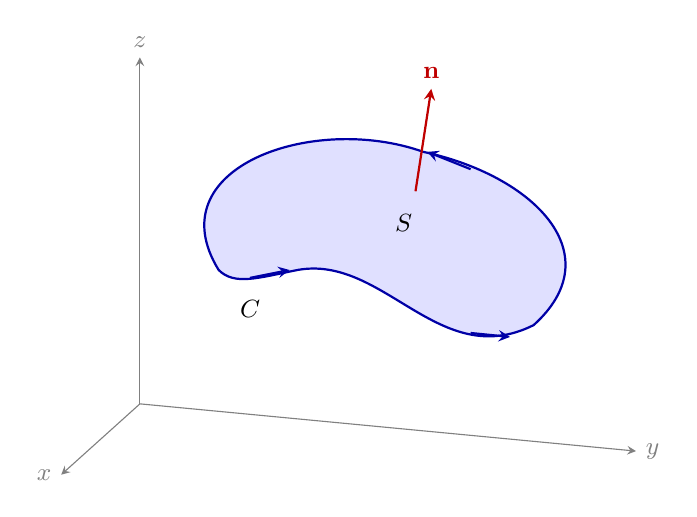
\begin{tikzpicture}[every node/.style={font=\small},>=stealth]

\draw[->,gray] (-3,-1.7)--(-3,2.7) node[above] {$z$};
\draw[->,gray] (-3,-1.7)--(3.3,-2.3) node[right] {$y$};
\draw[->,gray] (-3,-1.7)--(-4,-2.6) node[left] {$x$};
\fill[blue!12] (-2,0)..controls(-2.8,1.3)and(-.8,2)..(.6,1.5)
 ..controls(2,1.2)and(3,.2)..(2,-.7)
 ..controls(.8,-1.3)and(.1,.2)..(-1,0)..controls(-1.5,-.1)and(-1.8,-.2)..(-2,0);
\draw[blue!65!black,thick] (-2,0)..controls(-2.8,1.3)and(-.8,2)..(.6,1.5)
 ..controls(2,1.2)and(3,.2)..(2,-.7)
 ..controls(.8,-1.3)and(.1,.2)..(-1,0)..controls(-1.5,-.1)and(-1.8,-.2)..(-2,0);
\draw[->,blue!65!black,thick] (-1.6,-.1)--(-1.1,0);
\draw[->,blue!65!black,thick] (1.2,-.8)--(1.7,-.85);
\draw[->,blue!65!black,thick] (1.2,1.28)--(.65,1.5);
\draw[->,red!75!black,thick] (.5,1)--(.7,2.3) node[above] {$\mathbf n$};
\node at (.35,.6) {$S$}; \node at (-1.6,-.5) {$C$};

\end{tikzpicture}
\endgroup
\end{minipage}
\end{center}

Una superficie curva también induce un sentido de recorrido en su frontera. Las normales señalan el lado elegido de $S$ y las flechas azules siguen la orientación positiva de $C$.

\subsection{Enunciado del teorema}

Se consideran superficies compactas orientables que admiten una descomposición finita en parches regulares de clase $C^1$, con interiores disjuntos y fronteras suaves por partes. Las parametrizaciones tienen derivadas parciales primeras continuas y sus vectores tangentes son linealmente independientes. Las orientaciones de los parches son compatibles en las uniones. Esta clase incluye discos, porciones de planos, hemisferios y superficies formadas por varias caras.

\begin{mytheorem}{Teorema de Stokes}
Sea $S$ una superficie compacta, orientada y regular de clase $C^1$ por partes, del tipo descrito, y sea $C=\partial S$ su frontera suave por partes con la orientación inducida por $\mathbf n$. Si $\mathbf F$ es de clase $C^1$ en un abierto que contiene a toda $S$, entonces
\[
\oint_C\mathbf F\cdot d\vec r
=\iint_S(\nabla\times\mathbf F)\cdot\mathbf n\,dS.
\]
Si la frontera tiene varias componentes, la integral de línea representa la suma sobre todas ellas, cada una con su orientación inducida.
\end{mytheorem}

\begin{center}
\begin{minipage}{.94\textwidth}
\centering
\begingroup\shorthandoff{>}
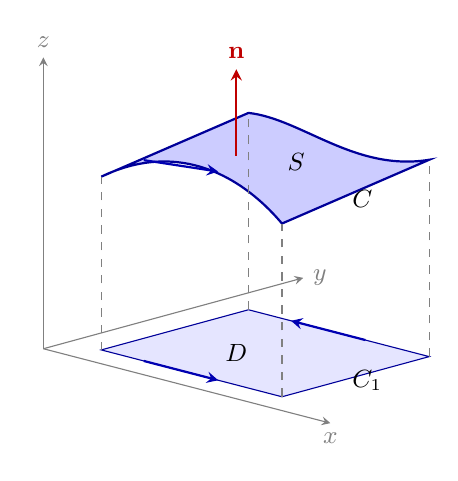
\begin{tikzpicture}[every node/.style={font=\small},>=stealth]

\begin{scope}[x={(1.35cm,-.35cm)},y={(1.1cm,.3cm)},z={(0cm,1cm)}]
\draw[->,gray] (0,0,0)--(2.7,0,0) node[below] {$x$};
\draw[->,gray] (0,0,0)--(0,3,0) node[right] {$y$};
\draw[->,gray] (0,0,0)--(0,0,3.7) node[above] {$z$};
\filldraw[fill=blue!10,draw=blue!60!black] (.3,.3,0)--(2,.3,0)--(2,2,0)--(.3,2,0)--cycle;
\filldraw[fill=blue!20,draw=blue!60!black,thick]
(.3,.3,2.2)..controls(1,.3,2.9)and(1.6,.3,2.7)..(2,.3,2.2)
--(2,2,2.5)..controls(1.3,2,2.1)and(.8,2,2.6)..(.3,2,2.5)--cycle;
\foreach \u/\v/\h in {.3/.3/2.2,2/.3/2.2,2/2/2.5,.3/2/2.5}
\draw[dashed,gray] (\u,\v,0)--(\u,\v,\h);
\draw[->,blue!70!black,thick] (.7,.3,0)--(1.4,.3,0);
\draw[->,blue!70!black,thick] (1.4,2,0)--(.7,2,0);
\draw[->,blue!70!black,thick] (.7,.3,2.55)--(1.4,.3,2.65);
\draw[->,red!75!black,thick] (1,1,2.5)--(1,1,3.6) node[above] {$\mathbf n$};
\node at (1,1,0) {$D$}; \node at (1.4,1.2,2.5) {$S$};
\node[right] at (2,1,2.3) {$C$}; \node[right] at (2,1,0) {$C_1$};
\end{scope}

\end{tikzpicture}
\endgroup
\end{minipage}
\end{center}

Para una gráfica $z=g(x,y)$ con normal ascendente, la frontera $C$ se proyecta sobre $C_1=\partial D$ con orientación antihoraria. Los segmentos punteados indican la proyección vertical; $C$ y $C_1$ son curvas distintas.

Si $S$ está en el plano $xy$, orientada por $\mathbf k=\langle0,0,1\rangle$, entonces
\[
(\nabla\times\mathbf F)\cdot\mathbf k=Q_x-P_y,
\qquad \mathbf F\cdot d\vec r=P\,dx+Q\,dy.
\]
Por tanto, Stokes se reduce a la forma de circulación de Green.

\subsection{Interpretación geométrica y física}

Geométricamente, cada parche aporta una circulación local. Al sumar sobre parches vecinos, los recorridos interiores se cancelan y queda únicamente la circulación de la frontera exterior y de los posibles orificios. La integral del rotacional acumula esas contribuciones con el signo determinado por la normal.

\begin{center}
\begin{minipage}{.94\textwidth}
\centering
\begingroup\shorthandoff{>}
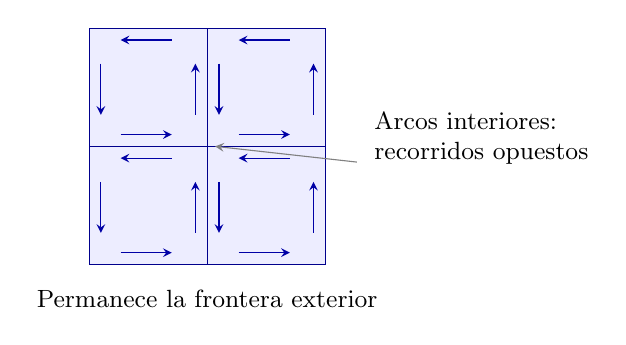
\begin{tikzpicture}[every node/.style={font=\small},>=stealth]

\foreach \a in {0,1} {\foreach \b in {0,1} {
\fill[blue!7] (\a*1.5,\b*1.5) rectangle ++(1.5,1.5);
\draw[blue!55!black] (\a*1.5,\b*1.5) rectangle ++(1.5,1.5);
\draw[->,blue!65!black] (\a*1.5+.4,\b*1.5+.15)--++(.65,0);
\draw[->,blue!65!black] (\a*1.5+1.35,\b*1.5+.4)--++(0,.65);
\draw[->,blue!65!black] (\a*1.5+1.05,\b*1.5+1.35)--++(-.65,0);
\draw[->,blue!65!black] (\a*1.5+.15,\b*1.5+1.05)--++(0,-.65);
}}
\node[align=left,anchor=west] at (3.5,1.6) {Arcos interiores:\\recorridos opuestos};
\draw[->,gray] (3.4,1.3)--(1.6,1.5);
\node[below] at (1.5,-.2) {Permanece la frontera exterior};

\end{tikzpicture}
\endgroup
\end{minipage}
\end{center}

Si $\mathbf F$ representa la velocidad de un fluido, su componente tangencial a una curva indica cuánto del movimiento sigue el contorno. Sea $S_\alpha$ un disco plano de radio $\alpha$, con centro $p$ y normal unitaria $\mathbf n$, y sea $C_\alpha$ su circunferencia orientada positivamente. En cada punto de $C_\alpha$, se denota por $\mathbf T$ la tangente unitaria en el sentido del recorrido.

El producto $\mathbf F\cdot\mathbf T$ es positivo cuando el fluido avanza en el sentido de $C_\alpha$, negativo cuando avanza en sentido contrario y cero cuando la velocidad es perpendicular a la tangente. Por ello, la integral
\[
\oint_{C_\alpha}\mathbf F\cdot\mathbf T\,ds
=\oint_{C_\alpha}\mathbf F\cdot d\vec r
\]
se llama circulación de $\mathbf F$ alrededor de $C_\alpha$. Suma las contribuciones tangenciales a lo largo de una vuelta completa.

\begin{center}
\begin{minipage}{.94\textwidth}
\centering
\begingroup\shorthandoff{>}
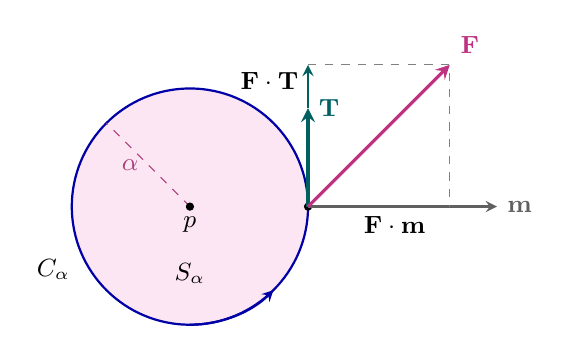
\begin{tikzpicture}[every node/.style={font=\small},>=stealth]
\filldraw[fill=magenta!10,draw=blue!65!black,thick] (0,0) circle (1.5);
\draw[->,blue!65!black,thick] (0,-1.5) arc(270:315:1.5);
\draw[dashed,magenta!65!black] (0,0)--(-1.06,1.06) node[midway,left] {$\alpha$};
\fill (0,0) circle (1.5pt) node[below] {$p$};
\node at (0,-.85) {$S_\alpha$};
\node[left] at (-1.4,-.8) {$C_\alpha$};
\coordinate (P) at (1.5,0);
\fill (P) circle (1.5pt);
\draw[->,teal!75!black,very thick] (P)--(1.5,1.25) node[right] {$\mathbf T$};
\draw[->,gray!75!black,thick] (P)--(3.9,0) node[right] {$\mathbf m$};
\draw[->,magenta!75!black,very thick] (P)--(3.3,1.8) node[above right] {$\mathbf F$};
\draw[dashed,gray] (1.5,1.8)--(3.3,1.8)--(3.3,0);
\draw[->,teal!75!black,thick] (1.5,1.25)--(1.5,1.8);
\node[left] at (1.5,1.6) {$\mathbf F\cdot\mathbf T$};
\node[below] at (2.6,0) {$\mathbf F\cdot\mathbf m$};
\end{tikzpicture}
\endgroup
\end{minipage}
\end{center}

Para estudiar el giro cerca de un punto $p$, se considera un disco $S_\alpha$ pequeño, contenido en el dominio del campo. Si el campo es de clase $C^1$, su rotacional varía poco en ese disco cuando $\alpha$ es suficientemente pequeño. Además, la normal $\mathbf n$ es constante porque el disco es plano. El teorema de Stokes da entonces
\begin{align*}
\oint_{C_\alpha}\mathbf F\cdot\mathbf T\,ds
&=\iint_{S_\alpha}(\nabla\times\mathbf F)\cdot\mathbf n\,dS\\
&\approx \bigl((\nabla\times\mathbf F)(p)\cdot\mathbf n\bigr)
\operatorname{area}(S_\alpha)\\
&=\bigl((\nabla\times\mathbf F)(p)\cdot\mathbf n\bigr)\pi\alpha^2.
\end{align*}
Por tanto,
\[
(\nabla\times\mathbf F)(p)\cdot\mathbf n
\approx\frac{\displaystyle\oint_{C_\alpha}\mathbf F\cdot\mathbf T\,ds}
{\pi\alpha^2}
=\frac{\text{circulación alrededor de }C_\alpha}
{\text{área del disco }S_\alpha}.
\]
Esta razón mide cuánto movimiento circulatorio se acumula por unidad de área. Al reducir el radio, la aproximación mejora y se obtiene la igualdad
\[
(\nabla\times\mathbf F)(p)\cdot\mathbf n
=\lim_{\alpha\to0^+}\frac{1}{\pi\alpha^2}
\oint_{C_\alpha}\mathbf F\cdot\mathbf T\,ds.
\]
Así, la componente normal del rotacional mide la circulación local por unidad de área respecto de la orientación $\mathbf n$.

\begin{center}
\begin{minipage}{.94\textwidth}
\centering
\begingroup\shorthandoff{>}
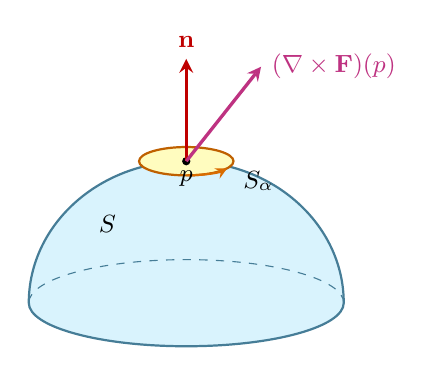
\begin{tikzpicture}[every node/.style={font=\small},>=stealth]
\fill[cyan!15] (-2,0) arc(180:0:2 and 1.8) arc(0:-180:2 and .55);
\draw[cyan!55!black,thick] (-2,0) arc(180:0:2 and 1.8);
\draw[cyan!55!black,dashed] (2,0) arc(0:180:2 and .55);
\draw[cyan!55!black,thick] (-2,0) arc(180:360:2 and .55);
\filldraw[fill=yellow!25,draw=orange!75!black,thick] (0,1.8) ellipse (.6 and .18);
\draw[->,orange!85!black,thick] (0,1.62) arc(270:330:.6 and .18);
\fill (0,1.8) circle (1.5pt) node[below] {$p$};
\draw[->,red!75!black,very thick] (0,1.8)--(0,3.1) node[above] {$\mathbf n$};
\draw[->,magenta!75!black,very thick] (0,1.8)--(.95,3) node[right] {$(\nabla\times\mathbf F)(p)$};
\node at (-1,1) {$S$};
\node[below right] at (.6,1.8) {$S_\alpha$};
\end{tikzpicture}
\endgroup
\end{minipage}
\end{center}

En un fluido, el campo $\boldsymbol\omega=\nabla\times\mathbf F$ se llama vorticidad. Si $\boldsymbol\omega(p)\cdot\mathbf n>0$, la circulación de discos suficientemente pequeños es positiva; si es negativa, predomina el giro contrario. Si la componente es cero, la circulación por unidad de área tiende a cero en esa dirección. Esto no significa que el fluido esté en reposo: una traslación uniforme tiene velocidad distinta de cero y rotacional nulo.

El teorema de Stokes reúne estas contribuciones locales: la circulación sobre la frontera de una superficie es igual al flujo de vorticidad a través de ella. Si $\mathbf F$ representa una fuerza, la misma integral de línea mide el trabajo realizado en una vuelta cerrada.

\paragraph{Ejemplo 1. Rotación alrededor de un eje}
El campo de velocidades de una rotación rígida alrededor del eje $z$ es
\[
\mathbf v=\langle-\omega_0 y,\omega_0 x,0\rangle,
\qquad \nabla\times\mathbf v=\langle0,0,2\omega_0\rangle,
\]
donde $\omega_0$ es la velocidad angular constante. En la circunferencia $C:x^2+y^2=a^2$, $z=0$, $a>0$, orientada en sentido antihorario visto desde arriba, Stokes da
\[
\oint_C\mathbf v\cdot d\vec r=\iint_{x^2+y^2\leq a^2}2\omega_0\,dA
=2\omega_0\pi a^2.
\]
Directamente, $\vec r(t)=\langle a\cos t,a\sin t,0\rangle$, $0\leq t\leq2\pi$, satisface
\[
\mathbf v(\vec r(t))\cdot\vec r\,'(t)=\omega_0 a^2,
\]
lo que produce el mismo resultado. La vorticidad es el doble de la velocidad angular dirigida en este movimiento; el signo de la circulación indica el sentido de giro respecto de la normal elegida.


\begin{center}
\begin{minipage}{.94\textwidth}
\centering
\begingroup\shorthandoff{>}
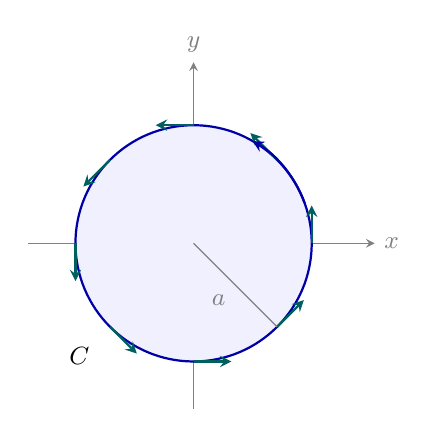
\begin{tikzpicture}[every node/.style={font=\small},>=stealth]

\draw[->,gray] (-2.1,0)--(2.3,0) node[right] {$x$};
\draw[->,gray] (0,-2.1)--(0,2.3) node[above] {$y$};
\fill[blue!6] (0,0) circle (1.5);
\draw[blue!65!black,thick] (0,0) circle (1.5);
\foreach \t in {0,45,...,315} {
\draw[->,teal!75!black,thick] ({1.5*cos(\t)},{1.5*sin(\t)})
 --++({-.48*sin(\t)},{.48*cos(\t)});}
\draw[->,blue!65!black,thick] ({1.5*cos(20)},{1.5*sin(20)}) arc(20:60:1.5);
\node[below left] at (-1.2,-1.2) {$C$};
\draw[gray] (0,0)--(1.06,-1.06) node[midway,below left] {$a$};
\end{tikzpicture}
\endgroup
\end{minipage}
\end{center}

\subsection{Elección de la superficie y ejemplos de aplicación}

Si dos superficies $S_1$ y $S_2$ tienen la misma frontera e inducen el mismo recorrido $C$, y el campo satisface las hipótesis en ambas, entonces
\[
\iint_{S_1}(\nabla\times\mathbf F)\cdot\mathbf n_1\,dS
=\oint_C\mathbf F\cdot d\vec r
=\iint_{S_2}(\nabla\times\mathbf F)\cdot\mathbf n_2\,dS.
\]

Para una gráfica $z=h(x,y)$ orientada hacia arriba se usa

\[
\mathbf n\,dS=\langle-h_x,-h_y,1\rangle\,dA.
\]

Para una parametrización orientada $\vec r(u,v)$ se usa $(\vec r_u\times\vec r_v)\,du\,dv$. En ambos casos, estos vectores incorporan el factor de área y no necesitan normalizarse.

\paragraph{Ejemplo 2. Circulación sobre una curva en un plano inclinado}
Sea $\mathbf F=\langle z,x,y\rangle$ y sea $C$ la intersección del cilindro $x^2+y^2=1$ con el plano $z=2-x-y$, recorrida de modo que su proyección sobre $xy$ sea antihoraria. El campo es de clase $C^1$ en $\mathbb R^3$ y
\[
\nabla\times\mathbf F=\langle1,1,1\rangle.
\]
La porción del plano sobre el disco unitario $D$ tiene normal ascendente y elemento dirigido $\mathbf n\,dS=\langle1,1,1\rangle\,dA$. Por tanto,
\[
\oint_C\mathbf F\cdot d\vec r
=\iint_D\langle1,1,1\rangle\cdot\langle1,1,1\rangle\,dA
=3\pi.
\]
La orientación indicada corresponde precisamente a la normal ascendente del plano.


\begin{center}
\begin{minipage}{.94\textwidth}
\centering
\begingroup\shorthandoff{>}
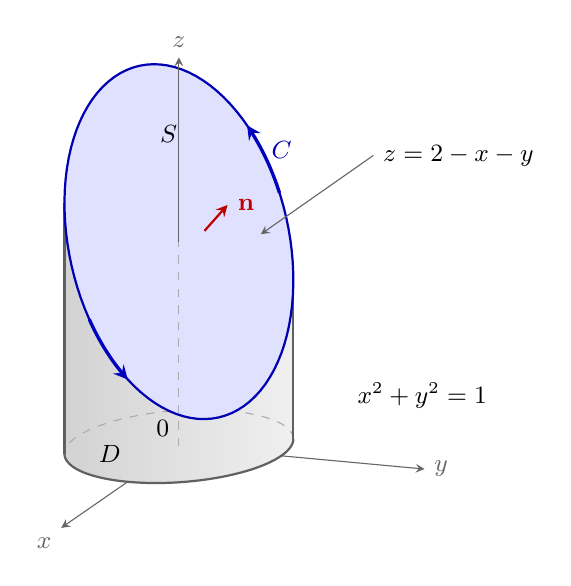
\begin{tikzpicture}[every node/.style={font=\small},>=stealth,
 x={(-.65cm,-.45cm)},y={(1.3cm,-.12cm)},z={(0cm,1.3cm)}]
% Ejes detrás del cilindro y región de proyección.
\draw[->,gray!80!black] (0,0,0)--(2.3,0,0) node[below left] {$x$};
\draw[->,gray!80!black] (0,0,0)--(0,2.4,0) node[right] {$y$};
\fill[gray!15] plot[domain=0:360,samples=81] ({cos(\x)},{sin(\x)},0)--cycle;
% Pared frontal del cilindro, recortada por el plano.
\shade[left color=gray!35,right color=gray!12]
 plot[domain=296.565:476.565,samples=51] ({cos(\x)},{sin(\x)},0)
 -- plot[domain=476.565:296.565,samples=51]
 ({cos(\x)},{sin(\x)},{2-cos(\x)-sin(\x)})--cycle;
% Frontera oculta y visible del disco inferior.
\draw[gray!65,dashed] plot[domain=116.565:296.565,samples=51]
 ({cos(\x)},{sin(\x)},0);
\draw[gray!75!black,thick] plot[domain=296.565:476.565,samples=51]
 ({cos(\x)},{sin(\x)},0);
\foreach \t in {116.565,296.565}
 \draw[gray!75!black,thick] ({cos(\t)},{sin(\t)},0)
 --({cos(\t)},{sin(\t)},{2-cos(\t)-sin(\t)});
% Superficie plana y su frontera orientada.
\filldraw[fill=blue!12,draw=blue!70!black,thick]
 plot[domain=0:360,samples=101]
 ({cos(\x)},{sin(\x)},{2-cos(\x)-sin(\x)})--cycle;
\draw[->,blue!75!black,very thick] plot[domain=335:360,samples=15]
 ({cos(\x)},{sin(\x)},{2-cos(\x)-sin(\x)});
\draw[->,blue!75!black,very thick] plot[domain=145:170,samples=15]
 ({cos(\x)},{sin(\x)},{2-cos(\x)-sin(\x)});
% Eje vertical y normal ascendente.
\draw[gray!65,dashed] (0,0,0)--(0,0,2);
\draw[->,gray!80!black] (0,0,2)--(0,0,3.8) node[above] {$z$};
\draw[->,red!75!black,thick] (-.2,.15,2.05)--(.25,.6,2.5)
 node[right] {$\mathbf n$};
\node at (-.5,-.35,2.85) {$S$};
\node at (.35,-.5,0) {$D$};
\node[above left] at (0,0,0) {$0$};
\node[right,blue!70!black] at (-.94,.34,2.6) {$C$};
\node[anchor=west] (plano) at (-.3,1.75,2.9) {$z=2-x-y$};
\draw[->,gray!80!black] (plano.west)--(-.5,.55,1.95);
\node[anchor=west] at (0,1.65,.65) {$x^2+y^2=1$};
\end{tikzpicture}
\endgroup
\par\smallskip
La pared del cilindro permite visualizar la proyección de $C$ sobre la frontera del disco $D$. La superficie de integración $S$ es la porción del plano inclinado; las flechas azules indican el recorrido compatible con la normal ascendente.
\end{minipage}
\end{center}

\paragraph{Ejemplo 3. Flujo del rotacional por un hemisferio}
Sea $S:x^2+y^2+z^2=4$, $z\geq0$, con normal radial exterior, y sea
\[
\mathbf F=\langle-y,x,z^2\rangle,
\qquad \nabla\times\mathbf F=\langle0,0,2\rangle.
\]
La frontera es $C:x^2+y^2=4$, $z=0$, orientada en sentido antihorario visto desde arriba. El disco $D$ en $z=0$, orientado por $\mathbf k$, induce ese mismo recorrido. Como el campo es regular en ambas superficies,
\[
\iint_S(\nabla\times\mathbf F)\cdot\mathbf n\,dS
=\iint_D2\,dA=8\pi.
\]
También se comprueba sobre la frontera: para $\vec r(t)=\langle2\cos t,2\sin t,0\rangle$ se tiene $\mathbf F(\vec r)\cdot\vec r\,'=4$, y su integral de $0$ a $2\pi$ es $8\pi$. El disco se orienta hacia arriba para aplicar Stokes; como tapa del semisólido en Gauss, su normal exterior sería hacia abajo.


\begin{center}
\begin{minipage}{.94\textwidth}
\centering
\begingroup\shorthandoff{>}
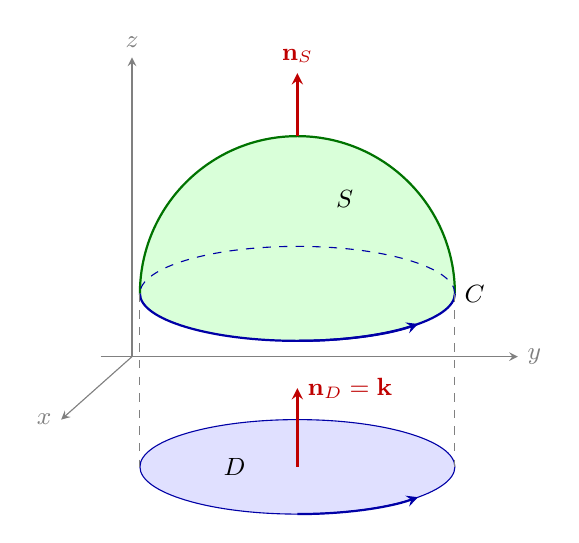
\begin{tikzpicture}[every node/.style={font=\small},>=stealth]

\draw[->,gray] (-2.5,-.8)--(2.8,-.8) node[right] {$y$};
\draw[->,gray] (-2.1,-.8)--(-2.1,3) node[above] {$z$};
\draw[->,gray] (-2.1,-.8)--(-3,-1.6) node[left] {$x$};
\fill[green!15] (-2,0) arc(180:0:2 and 2) arc(0:-180:2 and .6);
\draw[green!45!black,thick] (-2,0) arc(180:0:2 and 2);
\draw[blue!65!black,dashed] (2,0) arc(0:180:2 and .6);
\draw[blue!65!black,thick] (-2,0) arc(180:360:2 and .6);
\draw[->,blue!65!black,thick] (0,-.6) arc(270:320:2 and .6);
\draw[->,red!75!black,thick] (0,2)--(0,2.8) node[above] {$\mathbf n_S$};
\node at (.6,1.2) {$S$}; \node[right] at (2,0) {$C$};
\filldraw[fill=blue!12,draw=blue!65!black] (0,-2.2) ellipse (2 and .6);
\draw[->,blue!65!black,thick] (0,-2.8) arc(270:320:2 and .6);
\draw[->,red!75!black,thick] (0,-2.2)--(0,-1.2) node[right] {$\mathbf n_D=\mathbf k$};
\draw[dashed,gray] (-2,0)--(-2,-2.2); \draw[dashed,gray] (2,0)--(2,-2.2);
\node at (-.8,-2.2) {$D$};
\end{tikzpicture}
\endgroup
\end{minipage}
\end{center}

\paragraph{Ejemplo 4. Una superficie que no es plana}
Sea $S:z=1-x^2-y^2$, $x^2+y^2\leq1$, orientada hacia arriba, y sea $\mathbf F=\langle0,0,xy\rangle$. Se desea calcular el flujo de $\nabla\times\mathbf F$ a través de $S$ y comprobar su igualdad con la circulación sobre la frontera.

\begin{center}
\begin{minipage}{.94\textwidth}
\centering
\begingroup\shorthandoff{>}
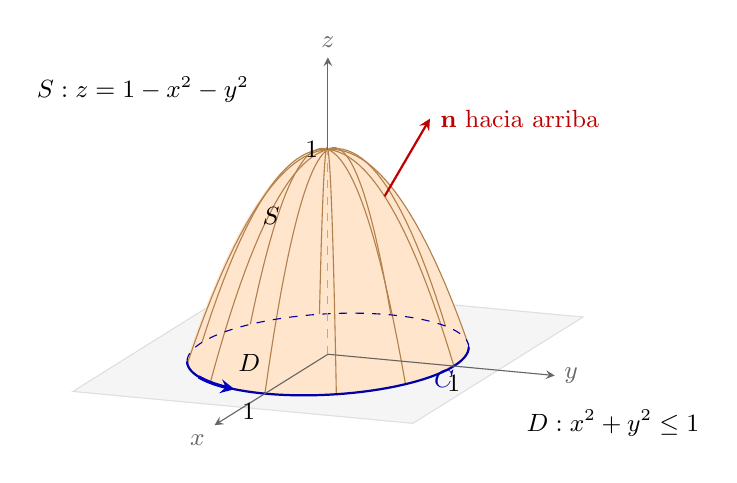
\begin{tikzpicture}[every node/.style={font=\small},>=stealth,
 x={(-.8cm,-.5cm)},y={(1.6cm,-.15cm)},z={(0cm,2.6cm)}]
\filldraw[fill=gray!8,draw=gray!25]
 (-1.35,-1.35,0)--(1.35,-1.35,0)--(1.35,1.35,0)--(-1.35,1.35,0)--cycle;
\fill[orange!14] plot[domain=0:360,samples=81] ({cos(\x)},{sin(\x)},0)--cycle;
% Meridianos y franjas de la superficie parabólica.
\foreach \t in {0,10,...,350} {
\fill[orange!20] plot[domain=0:1,samples=20]
 ({\x*cos(\t)},{\x*sin(\t)},{1-\x*\x})
 -- plot[domain=1:0,samples=20]
 ({\x*cos(\t+10)},{\x*sin(\t+10)},{1-\x*\x})--cycle;
}
\foreach \t in {0,30,...,330}
\draw[orange!40!gray,thin] plot[domain=0:1,samples=25]
 ({\x*cos(\t)},{\x*sin(\t)},{1-\x*\x});
\draw[blue!65!black,dashed] plot[domain=116.565:296.565,samples=51]
 ({cos(\x)},{sin(\x)},0);
\draw[blue!65!black,thick] plot[domain=296.565:476.565,samples=51]
 ({cos(\x)},{sin(\x)},0);
\draw[->,blue!75!black,very thick] plot[domain=320:345,samples=15]
 ({cos(\x)},{sin(\x)},0);
\draw[->,gray!80!black] (0,0,0)--(1.8,0,0) node[below left] {$x$};
\draw[->,gray!80!black] (0,0,0)--(0,1.8,0) node[right] {$y$};
\draw[gray!65,dashed] (0,0,0)--(0,0,1);
\draw[->,gray!80!black] (0,0,1)--(0,0,1.45) node[above] {$z$};
\node[left] at (0,0,1) {$1$};
\node at (0,-.45,.65) {$S$};
\node at (.35,-.45,0) {$D$};
\node[below] at (0,1,0) {$1$};
\node[below left] at (1,0,0) {$1$};
\node[right,blue!70!black] at (.35,.94,0) {$C$};
\draw[->,red!75!black,thick] (0,.45,.7975)--(0,.81,1.1975)
 node[right] {$\mathbf n$ hacia arriba};
\node[anchor=east] at (-.5,-.8,1.15) {$S:z=1-x^2-y^2$};
\node[anchor=west] at (0,1.5,-.25) {$D:x^2+y^2\leq1$};
\end{tikzpicture}
\endgroup
\end{minipage}
\end{center}

Para $P=Q=0$ y $R=xy$, el rotacional se obtiene por componentes:
\[
\nabla\times\mathbf F
=\left\langle
\frac{\partial(xy)}{\partial y}-0,\,
0-\frac{\partial(xy)}{\partial x},\,0-0
\right\rangle
=\langle x,-y,0\rangle.
\]
La superficie es la gráfica de $h(x,y)=1-x^2-y^2$ sobre $D$. Como $h_x=-2x$ y $h_y=-2y$, el elemento de superficie con orientación ascendente es
\[
\mathbf n\,dS=\langle-h_x,-h_y,1\rangle\,dA
=\langle2x,2y,1\rangle\,dA.
\]
Por tanto, el flujo se transforma en la integral doble
\begin{align*}
\iint_S(\nabla\times\mathbf F)\cdot\mathbf n\,dS
&=\iint_D\langle x,-y,0\rangle\cdot\langle2x,2y,1\rangle\,dA\\
&=\iint_D(2x^2-2y^2)\,dA.
\end{align*}
En coordenadas polares, $x=\rho\cos\theta$, $y=\rho\sin\theta$, con $0\leq\rho\leq1$ y $0\leq\theta\leq2\pi$. Se tiene $dA=\rho\,d\rho\,d\theta$ y $\cos^2\theta-\sin^2\theta=\cos(2\theta)$, de modo que
\begin{align*}
\iint_D(2x^2-2y^2)\,dA
&=\int_0^{2\pi}\int_0^1 2\rho^3\cos(2\theta)\,d\rho\,d\theta\\
&=\frac12\int_0^{2\pi}\cos(2\theta)\,d\theta\\
&=\left[\frac14\sin(2\theta)\right]_0^{2\pi}=0.
\end{align*}

Para verificar Stokes mediante la frontera, se parametriza $C$ con la orientación inducida:
\[
\vec r(t)=\langle\cos t,\sin t,0\rangle,
\qquad 0\leq t\leq2\pi.
\]
Sobre esta curva,
\[
\mathbf F(\vec r(t))=\langle0,0,\cos t\sin t\rangle,
\qquad \vec r\,'(t)=\langle-\sin t,\cos t,0\rangle.
\]
Su producto punto es cero porque el campo es vertical y la tangente es horizontal. En consecuencia,
\[
\oint_C\mathbf F\cdot d\vec r
=\int_0^{2\pi}0\,dt=0
=\iint_S(\nabla\times\mathbf F)\cdot\mathbf n\,dS.
\]
El rotacional no es nulo en toda la superficie, pero su flujo total se anula, como confirma la evaluación de la integral.

\subsection{Consecuencias y alcance}

Si $\nabla\times\mathbf F=\mathbf0$ en un entorno de una superficie admisible $S$, Stokes implica que la circulación sobre $\partial S$ es cero. Para concluir esto sobre una curva dada debe existir una superficie con esa frontera contenida en el dominio de regularidad.

\paragraph{Ejemplo 5. Una singularidad que impide usar un disco}
En $U=\{(x,y,z):x^2+y^2>0\}$, el campo
\[
\mathbf F=\left\langle-\frac{y}{x^2+y^2},\frac{x}{x^2+y^2},0\right\rangle
\]
tiene rotacional nulo. Sin embargo, para la circunferencia unitaria en $z=0$ recorrida en sentido antihorario,
\[
\mathbf F(\cos t,\sin t,0)\cdot\langle-\sin t,\cos t,0\rangle=1,
\qquad \oint_C\mathbf F\cdot d\vec r=2\pi.
\]
El disco atraviesa el eje $z$, donde el campo no está definido, así que Stokes no se aplica a él. Tampoco existe una superficie admisible contenida en $U$ con esa única frontera: si existiera, Stokes daría circulación cero, en contradicción con el cálculo. Por ello, rotacional nulo por sí solo no garantiza que un campo sea conservativo en cualquier dominio.


\begin{center}
\begin{minipage}{.94\textwidth}
\centering
\begingroup\shorthandoff{>}
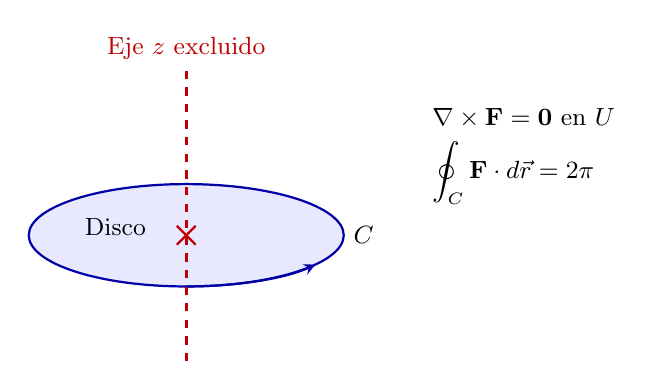
\begin{tikzpicture}[every node/.style={font=\small},>=stealth]

\fill[blue!9] (0,0) ellipse (2 and .65);
\draw[blue!65!black,thick] (0,0) ellipse (2 and .65);
\draw[->,blue!65!black,thick] (0,-.65) arc(270:325:2 and .65);
\draw[red!75!black,dashed,very thick] (0,-1.6)--(0,2.1) node[above] {Eje $z$ excluido};
\draw[red!75!black,thick] (-.12,-.12)--(.12,.12) (-.12,.12)--(.12,-.12);
\node[right] at (2,0) {$C$};
\node at (-.9,.1) {Disco};
\node[anchor=west,align=left] at (3,1) {$\nabla\times\mathbf F=\mathbf0$ en $U$\\[4pt]$\displaystyle\oint_C\mathbf F\cdot d\vec r=2\pi$};

\end{tikzpicture}
\endgroup
\end{minipage}
\end{center}

\subsection{Ejercicios}
\begin{enumerate}
    \item Determine la orientación inducida en la frontera de cada superficie: el disco $x^2+y^2\leq4$, $z=0$, con normal $-\mathbf k$; el hemisferio $x^2+y^2+z^2=4$, $z\geq0$, con normal radial exterior; y la corona plana $1\leq x^2+y^2\leq4$, $z=0$, con normal $\mathbf k$. Describa los recorridos vistos desde el semieje positivo $z$.

    \item Calcule el rotacional de $\mathbf F=\langle-y,x,z\rangle$ y use Stokes para evaluar su circulación sobre $x^2+y^2=9$, $z=0$, en sentido antihorario visto desde arriba.

    \item Evalúe $\oint_C\mathbf F\cdot d\vec r$ para $\mathbf F=\langle y,z,x\rangle$, donde $C$ recorre sucesivamente los vértices $(0,0,0)$, $(1,0,0)$, $(0,1,0)$ y $(0,0,0)$. Verifique el resultado mediante parametrizaciones de los tres segmentos.

    \item Use Stokes para calcular la circulación de $\mathbf F=\langle-y,x,xy\rangle$ sobre la intersección de $x^2+y^2=4$ con $z=3-x$, cuya proyección sobre $xy$ se recorre en sentido antihorario.

    \item Calcule $\iint_S(\nabla\times\mathbf F)\cdot\mathbf n\,dS$ para $\mathbf F=\langle-yz,xz,x^2+y^2\rangle$, donde $S$ es el hemisferio $x^2+y^2+z^2=4$, $z\geq0$, con orientación radial exterior. Use su frontera y una superficie plana con orientación compatible.

    \item Sea $\mathbf F=\langle z,0,x\rangle$ y sea $S:z=xy$, $0\leq x,y\leq1$, orientada hacia arriba. Verifique Stokes calculando tanto el flujo del rotacional como la circulación sobre los cuatro arcos de la frontera.

    \item Un fluido tiene velocidad $\mathbf v=\langle-\alpha y,\alpha x,\beta z\rangle$, donde $\alpha$ y $\beta$ son constantes. Determine la circulación sobre la intersección de $x^2+y^2=a^2$, $a>0$, con $z=h+mx+ny$, orientada con proyección antihoraria sobre $xy$. Interprete qué parámetros influyen en la circulación y relacione el resultado con la vorticidad.

    \item Sea $S$ la superficie lateral del cilindro $x^2+y^2=a^2$, $0\leq z\leq h$, con $a,h>0$ y normal radial exterior, y sea $\mathbf F=\langle-yz,xz,0\rangle$. Determine las orientaciones inducidas en las dos circunferencias de la frontera y verifique Stokes mediante el flujo del rotacional y la suma de las dos circulaciones.

    \item Sea $\mathbf F=\langle-y/(x^2+y^2),x/(x^2+y^2),0\rangle$. Verifique Stokes sobre la corona $a^2\leq x^2+y^2\leq b^2$, $z=0$, con $0<a<b$ y normal ascendente. Explique por qué no se puede sustituir la corona por el disco $x^2+y^2\leq b^2$ para conservar únicamente la frontera exterior.

    \item Sean $f$ y $g$ funciones escalares de clase $C^2$ en un abierto que contiene a $S$, y suponga que $C=\partial S$ y $S$ satisfacen las condiciones del teorema de Stokes, con orientaciones compatibles. Verifique cada una de las identidades siguientes:
\begin{enumerate}
\item $\displaystyle\oint_C(f\nabla g)\cdot d\vec r
=\iint_S(\nabla f\times\nabla g)\cdot\mathbf n\,dS$.
\item $\displaystyle\oint_C(f\nabla f)\cdot d\vec r=0$.
\item $\displaystyle\oint_C(f\nabla g+g\nabla f)\cdot d\vec r=0$.
\end{enumerate}

    \item Sea $\mathbf c$ un vector constante y sea $S$ una superficie orientada con normal unitaria $\mathbf n$, limitada por una curva $C=\partial S$, que satisface las hipótesis geométricas del teorema de Stokes. Oriente $C$ de manera compatible y demuestre que
\[
\iint_S\mathbf c\cdot\mathbf n\,dS
=\frac12\oint_C(\mathbf c\times\vec r)\cdot d\vec r,
\qquad \vec r=\langle x,y,z\rangle.
\]

\end{enumerate}
